\documentclass{article}
\usepackage{graphicx}
\usepackage{hyperref}
\usepackage{listings}
\usepackage{xcolor}
\usepackage{tikzsymbols}

\lstset{
    basicstyle=\ttfamily,
    backgroundcolor=\color{gray!30},
}

\begin{document}

\graphicspath{ {./Images/} }
\tableofcontents

\section{Introduction}
Hello and welcome to Windows. This document describes the process of configuring windows machines to run on Proxmox. If you would like to add something, please contribute in the github.

\section{Getting the correct ISOs to Proxmox}
The goal is to get both the Windows Server and the VirtIO driver iso files onto proxmox.

You should can either download the files to your computer and then to proxmox, or you can have proxmox download them from "download from url."

In either case, the Windows Server 2019 iso is \href{http://www.microsoft.com/en-us/evalcenter/download-windows-server-2019
}{here} and the VirtIO iso is \href{https://fedorapeople.org/groups/virt/virtio-win/direct-downloads/stable-virtio/}{here}.

The VirtIO is necessary because proxmox says so (update with better reasoning). \href{https://pve.proxmox.com/wiki/Windows_VirtIO_Drivers#Windows_OS_Support}{Proxmox Wiki: Windows VirtIO Drivers}

VirtIO also enables the QEMU Guest Agent, which allows for many convenient things in proxmox.

\begin{figure}[h]
    \centering
    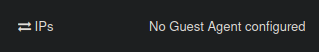
\includegraphics[width=0.5\textwidth]{noGuestAgent.png}
    \caption{The IP Address is not displayed if there is no guest agent}
    \label{fig:noGuestAgent}
\end{figure}

\section{Getting the VM from the ISO}
The goal is to take your .iso file and turn it into a VM. If it is helpful, here is some guy doing it with no words: \href{https://www.youtube.com/watch?v=lwORpWEHiDE&t=5m}{video} 

\noindent If you don't want to watch that, click "create VM" and select the iso file you uploaded.
\noindent The important settings to change are:
\vspace{1cm}

\begin{tabular}{l l}
    Category & Setting to Change\\
    \hline
    OS Type & Microsoft Windows, Version: 10/2016/2019 \\
    System & SCSI Controller: VirtIO SCSI Single \\
    System & QEMU Agent checked \\
    Disks & Bus/Device: SCSI \\
  \end{tabular}

After creating this VM, click it and go to the “Hardware” menu in Proxmox. Click “add CD/DVD” and click the virtIO.iso file you uploaded. This will enable the QEMU Agent.

\section{Installing / Logging Into the VM}
Note: You can not use many of proxmox's features (i.e. shut it down without going through the console) without the guest agent installed. Just to save you from mashing the "shutdown" button and wondering why it doesn't work. 

\noindent How to get into the VM:

\begin{enumerate}
    \item Power on the VM
    \item Log onto the VM via the Proxmox console
\end{enumerate}

\noindent How to install Windows on the VM:

\begin{enumerate}
    \item Select "next"
    \item Select "2019 Standard Evaluation (Desktop Experience)"
    \item Select "Advanced Installation"
    \item Add the VirtIO driver you installed previously
\end{enumerate}

Now you wait for it to install. Don't worry, you'll get used to waiting for windows!

\section{Basic Configurations to Prepare for a Template}
The goal is to never do that time consuming process again. We would like to create a template so we can clone it. Before you make a template you can add useful things like RDP, Firefox, setting DNS, etc. The world is your oyster.

\subsection{Installing Firefox}
By default, Internet Explorer is the only browser installed on the computer. What a terrible browser! You can avoid ever opening IE by installing Firefox from powershell. 
\begin{lstlisting}
    Invoke-WebRequest -Uri 
    "https://download.mozilla.org/
    ?product=firefox-msi-latest-ssl
    &os=win64&lang=en-US" 
    -OutFile "$HOME\Desktop\firefox.msi"
\end{lstlisting}

\noindent This command saves firefox.msi to your desktop. YRemember that you can download stuff from powershell. (But pls no proprietary browsers \Vomey{})

\end{document}
